
%
%  $Description: Author guidelines and sample document in
%  LaTeX 2.09$ 
%
%  $Author: ienne $ $Date: 1995/09/15 15:20:59 $ $Revision:
%  1.4 $
%

\documentclass[times, 10pt,twocolumn]{article}
\usepackage{latex8} \usepackage{times}
\usepackage{graphicx}

%\documentstyle[times,art10,twocolumn,latex8]{article}

\newcommand{\forceindent}{\leavevmode{\parindent=1em\indent}}

%-------------------------------------------------------------------------
%take the % away on next line to produce the final
%camera-ready version 
\pagestyle{empty}

%------------------------------------------------------------------------- 
\begin{document}

\title{\ Distributed and Fault-Tolerant System for Tuple
Streaming}

			 \author{Jorge Santos, Miguel Vera, Jos\'e Semedo \\
				 Instituto Superior Tecnico\\ Computer Science
				 Department\\ ??IN-F??  Av. Rovisco Pais, 1,
				 1049-001 Lisboa\\ \{jorge.pessoa, miguel.vera,
				 jose.semedo\}@tecnico.ulisboa.pt }

\maketitle \thispagestyle{empty}

\begin{abstract} The ABSTRACT is to be in fully-justified
	italicized text, at the top of the left-hand column, below
	the author and affiliation information.  Use the word
	``Abstract'' as the title, in 12-point Times, boldface
	type, centered relative to the column, initially
	capitalized. The abstract is to be in 10-point,
	single-spaced type.  The abstract may be up to 3 inches
	(7.62 cm) long. Leave two blank lines after the Abstract,
	then begin the main text.  \end{abstract}



%------------------------------------------------------------------------- 
\Section{Introduction}

Please follow the steps outlined below when submitting your
manuscript to the IEEE Computer Society Press. Note there
have been some changes to the measurements from previous
instructions. 

%------------------------------------------------------------------------- 
\Section{Solutions}

Describe the solutions in an overall way

%------------------------------------------------------------------------- 
\SubSection{Solution 1}

Solution 1 advantages/disadvantages

%------------------------------------------------------------------------- 
\SubSection{Solution 2}

Solution 1 advantages/disadvantages

%------------------------------------------------------------------------- 
\Section{Fault-Tolerance}

Talk about fault-tolerance in a general way

Our fault tolerance algorithm provides the ability to tolerate a downed replica of any operator, as well as the it's recuperation.
The algorithm we used is possible due to the use of a simple, yet resourceful abstraction mechanism, which the semanthics algorithm will greatly benefit from aswell.
Each of the replica mantains three sets of of dictionaries, except the first and last operator's replicas. This is because each of the dictionaries holds the correspondence between a replica and the dictionary holder's view of it.
One dictionary abstracts all of the colleague replicas of the holder (replicas of the same operator as itself), another distinct dictionary abstracts the replicas of the above operator, and again for the one below.
So every replica of every operator has the ability to establish a connection with what they think is every replica above and below them, as well as their colleagues.

%------------------------------------------------------------------------- 
\SubSection{Fault Detection}

Going into more detail on how a downed replica can be detected.
Colleague replicas among themselves have the illusion of being in a ring like topology. Each replica periodically pings the following colleague like ilustrated in fig.X (FIGURA DE REPLICAS EM CIRCULO COM INDEXES E SETAS DE PING). A replica can efficiently know what replica it preceeds. It knows it's own replica index (i)therefor it knows the index of the replica it has to ping (ping i), by applying the following rule: ping i = (i + 1) \% number of replicas.
If the pinged replica is detected to be down, then the replica can just calculate the following replica's index using the very same rule, and contact it, asking for it to take over the downed replica's spot.
\begin{figure}[h] 
	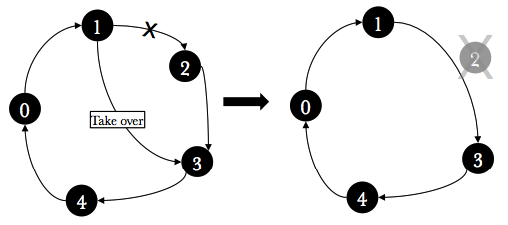
\includegraphics[width=\columnwidth]{fault_detection}
	\caption{Ordered steps taken when a node processes a tuple}
\end{figure}

%------------------------------------------------------------------------- 
\SubSection{Take Over Procedure}

The replica taking over goes through the 3 sets of replica holding abstractions aforementioned.
Firstly it iterates over the the replica holding abstractions corresponding to the operator above it, and for each one, it substitues the place of the replica detected as downed with a representation of itself. It literally takes over it's spot, so every command that would be aimed at the downed replica, is routed to the one that took over it's functions.
It then repeats the process for it's colleague replicas and the ones of the operator below it. (FIGURA COM SETAS E O CRLH)

\begin{figure}[h] 
	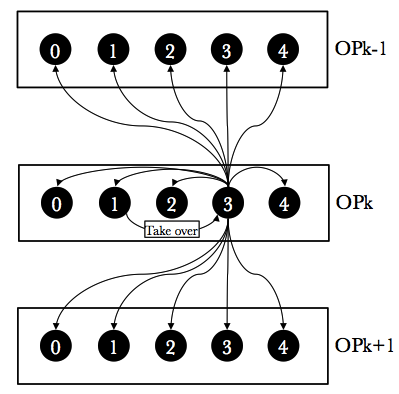
\includegraphics[width=\columnwidth]{take_over}
	\caption{Ordered steps taken when a node processes a tuple}
\end{figure}

There is however a small detail that caused a somewhat meaningful problem. In the case of an operator having only two replicas, and one of them going down, the only remaining replica would substitute the representation of it's colleague with itself, and then effectively start pinging itself. This caused not only some perfformance issues but some other problems.
In order to fix this efficiently we had to break a small layer of abstraction and add another sctructure to the replicas, a list containing the indexes of the replicas it has taken over. This allows a replica to know whether it would be connecting to itself or not.

After a replica has fully taken over for another one, all other replicas have the illusion of the topology state remaining the same. This is because every method that implies connecting to another replica, obtains the connection through the abstraction layer previously described, so every work load is seamlessly diverted to the new replica.
Only replicas within the same operator can detect downed replicas. If any other remoting method fails due to the target replica being down, it enters an active wait untill another replica takes over and the method is succesfully carried out. We chose this implementation over the option of any remoting task possibly triggering a take over, due to the possibility of the retrying of the faulting method being faster than the take over process. Fixing this issue would over complicate things, and the simpler implementation as we have now would reveal it self as the faster one.
%------------------------------------------------------------------------- 
\SubSection{Reinstate Procedure}

The reinstating protocol is simply put, the reverse of the take over process. Once a replica is brought back it goes through the same process of accessing previous, colleague and following operator's replica abstraction holding structures in that respoecting order, and inserting a representation of itself in it's rightful spot.
After this, all remote methods are once again routed correctly to the reinstated replica.
The replica that had taken over for it also has it's index list updated, meaning that the index of the reinstated replica is removed from that list.
%------------------------------------------------------------------------- 
\Section{Semantics}

One of the biggest concern in the distributed tuple processing is being
able to a guarantee a certain semantics associated with the processing of
a tuple in the presence of system failures, and inevitably the way in
needs to reconfigure in order to continue functioning properly. This issue
is inevitably linked to the way that the system does fault tolerance. The
algorithm used for any semantic guarantee is very simillar, using 
the same data structures and most of the same procedures,
We will first explain the general idea behind the algorithm, then used data structures and the algorithm and
finally how it used to assure that a tuple is processed at most once,
at least once and exactly once.

%------------------------------------------------------------------------- 
\SubSection{Explanation}


If the system
must process a certain tuple at least once then there must a guarantee
that in any kind of a node failure the tuples that weren't successfuly
sent to a node in failure are sent either to another node or to the the
original node if it recovers. There are however other scenarios in which a
node can fail, For example after receiving a tuple but before sending it
to the next operator. Keeping in mind that the system must
obviously be ashynchronous in this confirmation, then the previous node
can't easily know it has to resend the tuple, and when it doesn't, or how
long it needs to keep the tuple.  In this approach the tuples would need
to be kept in every operator at least until the tuple was processed by
every node, presenting scalability issues. That's why we opted to use
an algorithm based in keeping the information of the tuples being processed
and by which replica, as well as which replica originally contains the tuple.
That way all the tuples that weren't sent can be processed and sent again
if a new node takes over a dead node without the need to replica tuples by
all nodes of an operator.

%------------------------------------------------------------------------- 
\SubSection{Data Structures}


To understand how the
algorithm works we must first explain the used data structures: A tuple is
identified by it's Tuple Id structure which represents a stream of a tuple
along the processing chain. In each specific tuple there is an unique id
that is usualy kept along all operators, unless there must an output of
several tuples from the same one, efectively diverging the tuple stream.
The remaining information kept in the Tuple Id refers to the operator and
replica it came from. 

In each node there is a delivery table (a simple
Hash-based Map that stores each tuple by its unique id) and that keeps
every tuple received in a replica until it can be disposed.  

There is
also a shared tuple table in each node that stores Tuple Records
associated to a tuple id (in a simillar Hash Map). A tuple record is a
small representation of a tuple containing its Tuple Id, as well as the
replica emiting the tuple record. This way the tuple record contains only
the necessary information for a node to re-process a tuple that wasn't
properly processed due to failure. For information storing purposes the
tuple records have a state (pending or purged) that is used to store
tuple records of the tuples processed by a replica in a purged state
instead of deleting them in order to properly know what tuples have
already been processed by that replica.


%------------------------------------------------------------------------- 
\SubSection{Algorithm}

\begin{figure}[h] 
	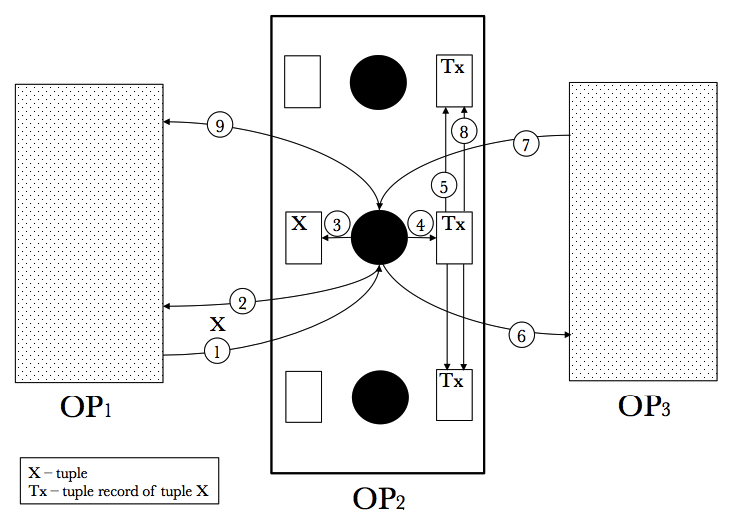
\includegraphics[width=\columnwidth]{semantics}
	\caption{Ordered steps taken when a node processes a tuple}
\end{figure}

The ordered steps represented in figure 1 show most of the necessary 
procedures executed every time a tuple is received, to keep the data structures synchronized in order to allow a
proper recovery when a node fails. When a node receives a tuple (1) the first
thing it must do is insert it into it's delivery table (2) and it's shared tuple
record table (3). The node then synchronizes every table with other replicas
shared tables (4) and finnaly processes the tuple, sending it afterwards (5). After the
tuple is sent and confirmation is received (6) the node will first issue the
deletion of the tuple record of every other shared table and purge its own
shared table of the same tuple (7). Finally it will warn the replica which the
tuple originated from that it can finally delete it from its delivery table (8)
since it was already received by the forward node. This information is
used whenever a node takes over another failling node. It scans its shared
table looking for tuple records of the dead node and for each record it finds,
it requests the tuple to the replica that the tuple originated from. Finally that tuple is
processed and sent to the following node, by the same procedures explained
before, as if a new tuple was received. 

Note that this approach only
ensures the semantics of the delivery in case of a single horizontal
failure (when two sequential replicas on the path of processing a tuple
fail). It could also support more failures if necessary by extending the
number of nodes where a tuple is kept before it is delivered.

%------------------------------------------------------------------------- 
\SubSection{Differences for each guarantee}



%------------------------------------------------------------------------- 
\subsubsection{At-Most-Once}

\forceindent To assure that a tuple is processed at most once, a system must only send
any tuple once, indepent of failure. Since a configuration for this system
is dependent on being an acyclic graph, the only guarantee we need to
provide is that there isn't any kind of mechanism to resend tuples in case
of a takeover of a node that crashed by another node.  As such the
implementation of this strategy relies on not sharing any kind of
information about tuples already processed, which is achieved by not executing
any kind of the procedures explained before related to the applied algorithm
(that isn't really applied in this case of semantics).
This way, a certain tuple from an input is only sent once in
the forward direction of the distributed network, and in case of a node
failing all the tuples that it had processed but not sent yet won't be
processed at all. The same applies to a replica that sends a tuple to the next
replica, which in case of not getting a response, will just drop the tuple.

%------------------------------------------------------------------------- 
\subsubsection{At-Least-Once}

\forceindent The algorithm previously basicaly accomplishes at least once
delivery by itself, without the need of any changes. 

%------------------------------------------------------------------------- 
\subsubsection{Exactly-Once}

\forceindent Finally to guarantee that tuples are delivered only exactly once, and taking
the algorithm descbibed as a starting point, there is the need to guarantee
that a tuple is never processed twice on the same operator. The first thing
to remember is that each tuple has a unique Id that identifies it's path
along the processing chain. Based on that, each received tuple on a node is
checked by it's id to guarantee that it has never been processed, by comparing
it's unique id to every tuple record stored in the shared tuple record table
(hence the possible states for a certain tuple).
The tuple is accepted with success in case it was never inserted in the table,
assuring the replica that the tuple was never processed and sent to next
operator before, which together with the guarantees provided by the algorithm
assure exactly once delivery of tuples.

%------------------------------------------------------------------------- 
\Section{Evaluation}

Evaluation of the solution

%------------------------------------------------------------------------- 
\SubSection{Quantitative}

Quantitive evaluation

%------------------------------------------------------------------------- 
\SubSection{Qualitative}

Qualitative evaluation

%------------------------------------------------------------------------- 
\Section{Discussion}

Prior to analyzing the used algorithms, we have to acknowledge that the
solutions aren't perfect but are a step forward from the naive approaches
that might be picked in this situation. Most of the differences are actually
?intelligible? when processing small datasets, in which each tuple is small.
For example in this case there is an advantage of replicating tuples in each
node after receiving from the operator, considering their sizes might be even
smaller than the tuple records and there are less steps involved in the
algorithm. But on the other hand, if we try to scale the tuple size even
a little bit, then the tuple-replicating approach would scale much worse,
resulting in huge amounts of exchanged data between replicas of the same
operator before they can even process the tuples. On the other hand, replicating
only tuple records scales in a constant way with tuple size (doesn't increase).
So as analyzed from this feature, one thing to note is that there is no perfect
solution that applies to every kind of system in a scallable and eficient way.
A much better compromise is to develop the system according to whatever are
its needs, and if possible without forgetting the scalability to a real world
scenario of applying the developed solution.

%------------------------------------------------------------------------- 
\Section{Conclusion}

Evaluation of the solution

%------------------------------------------------------------------------- 
\Section{Style Guidelines}

Please follow the steps outlined below when submitting your manuscript to
the IEEE Computer Society Press. Note there have been some changes to the
measurements from previous instructions. 

%------------------------------------------------------------------------- 
\SubSection{Margins and page numbering}

All printed material, including text, illustrations, and charts, must be
kept within a print area 6-7/8 inches (17.5 cm) wide by 8-7/8 inches
(22.54 cm) high.  Do not write or print anything outside the print area.
Number your pages lightly, in pencil, on the upper right-hand corners of
the BACKS of the pages (for example, 1/10, 2/10, or 1 of 10, 2 of 10, and
so forth). Please do not write on the fronts of the pages, nor on the
lower halves of the backs of the pages.


%------------------------------------------------------------------------ 
\SubSection{Formatting your paper}

All text must be in a two-column format. The total allowable width of the
text area is 6-7/8 inches (17.5 cm) wide by 8-7/8 inches (22.54 cm) high.
Columns are to be 3-1/4 inches (8.25 cm) wide, with a 5/16 inch (0.8 cm)
space between them.  The main title (on the first page) should begin 1.0
inch (2.54 cm) from the top edge of the page. The second and following
pages should begin 1.0 inch (2.54 cm) from the top edge. On all pages, the
bottom margin should be 1-1/8 inches (2.86 cm) from the bottom edge of the
page for $8.5 \times 11$-inch paper; for A4 paper, approximately 1-5/8
inches (4.13 cm) from the bottom edge of the page.

%------------------------------------------------------------------------- 
\SubSection{Type-style and fonts}

Wherever Times is specified, Times Roman may also be used.  If neither is
available on your word processor, please use the font closest in
appearance to Times that you have access to.

MAIN TITLE. Center the title 1-3/8 inches (3.49 cm) from the top edge of
the first page. The title should be in Times 14-point, boldface type.
Capitalize the first letter of nouns, pronouns, verbs, adjectives, and
adverbs; do not capitalize articles, coordinate conjunctions, or
prepositions (unless the title begins with such a word).  Leave two blank
lines after the title.

AUTHOR NAME(s) and AFFILIATION(s) are to be centered beneath the title and
printed in Times 12-point, non-boldface type.  This information is to be
followed by two blank lines.

The ABSTRACT and MAIN TEXT are to be in a two-column format. 

MAIN TEXT. Type main text in 10-point Times, single-spaced.  Do NOT use
double-spacing. All paragraphs should be indented 1 pica (approx. 1/6 inch
or 0.422 cm). Make sure your text is fully justified---that is, flush left
and flush right.  Please do not place any additional blank lines between
paragraphs.  Figure and table captions should be 10-point Helvetica
boldface type as in \begin{figure}[h] \caption{Example of caption.}
\end{figure}

\noindent Long captions should be set as in \begin{figure}[h]
	\caption{Example of long caption requiring more than one line. It is not
	typed centered but aligned on both sides and indented with an additional
margin on both sides of 1~pica.} \end{figure}

\noindent Callouts should be 9-point Helvetica, non-boldface type.
Initially capitalize only the first word of section titles and first-,
second-, and third-order headings.

FIRST-ORDER HEADINGS. (For example, {\large \bf 1.  Introduction}) should
be Times 12-point boldface, initially capitalized, flush left, with one
blank line before, and one blank line after.

SECOND-ORDER HEADINGS. (For example, {\elvbf 1.1. Database elements})
should be Times 11-point boldface, initially capitalized, flush left, with
one blank line before, and one after. If you require a third-order heading
(we discourage it), use 10-point Times, boldface, initially capitalized,
flush left, preceded by one blank line, followed by a period and your text
on the same line.

%------------------------------------------------------------------------- 
\SubSection{Footnotes}

Please use footnotes sparingly% \footnote {% Or, better still, try to
	avoid footnotes altogether.  To help your readers, avoid using footnotes
	altogether and include necessary peripheral observations in the text
	(within parentheses, if you prefer, as in this sentence). and place them
	at the bottom of the column on the page on which they are referenced.
	Use Times 8-point type, single-spaced.


%------------------------------------------------------------------------- 
\SubSection{References}

List and number all bibliographical references in 9-point Times,
single-spaced, at the end of your paper. When referenced in the text,
enclose the citation number in square brackets, for example~\cite{ex1}.
Where appropriate, include the name(s) of editors of referenced books.

%------------------------------------------------------------------------- 
\SubSection{Illustrations, graphs, and photographs}

All graphics should be centered. Your artwork must be in place in the
article (preferably printed as part of the text rather than pasted up).
If you are using photographs and are able to have halftones made at a
print shop, use a 100- or 110-line screen. If you must use plain photos,
they must be pasted onto your manuscript. Use rubber cement to affix the
images in place. Black and white, clear, glossy-finish photos are
preferable to color. Supply the best quality photographs and illustrations
possible. Penciled lines and very fine lines do not reproduce well.
Remember, the quality of the book cannot be better than the originals
provided. Do NOT use tape on your pages!

%------------------------------------------------------------------------- 
\SubSection{Color}

The use of color on interior pages (that is, pages other than the cover)
is prohibitively expensive. We publish interior pages in color only when
it is specifically requested and budgeted for by the conference
organizers. DO NOT SUBMIT COLOR IMAGES IN YOUR PAPERS UNLESS SPECIFICALLY
INSTRUCTED TO DO SO.

%------------------------------------------------------------------------- 
\SubSection{Symbols}

If your word processor or typewriter cannot produce Greek letters,
mathematical symbols, or other graphical elements, please use
pressure-sensitive (self-adhesive) rub-on symbols or letters (available in
most stationery stores, art stores, or graphics shops).

%------------------------------------------------------------------------ 
\SubSection{Copyright forms}

You must include your signed IEEE copyright release form when you submit
your finished paper. We MUST have this form before your paper can be
published in the proceedings.

%------------------------------------------------------------------------- 
\SubSection{Conclusions}

Please direct any questions to the production editor in charge of these
proceedings at the IEEE Computer Society Press: Phone (714) 821-8380, or
Fax (714) 761-1784.

%------------------------------------------------------------------------- 
\nocite{ex1,ex2} \bibliographystyle{latex8} \bibliography{latex8}

\end{document}

